% Scalar instruction entry source: tools/generate_scalar_instruction_catalog.py.
\subsection{\texttt{LR.W}}
\label{sec:scalar-lr_w}
\index{LR.W@\texttt{LR.W}}
\begin{sloppypar}\noindent\textbf{Purpose.} Load-reserved: performs an atomic load and establishes a reservation for a subsequent store-conditional.\end{sloppypar}\smallskip
\noindent\textbf{Syntax.}\par
\begin{lstlisting}[style=ptoscalarcode]
lr.w<.{aq, rl, f, aqrl, aqf, rlf, aqrlf}> [SrcL], ->RegDst
\end{lstlisting}
\noindent\textbf{Encoding.}\par
\noindent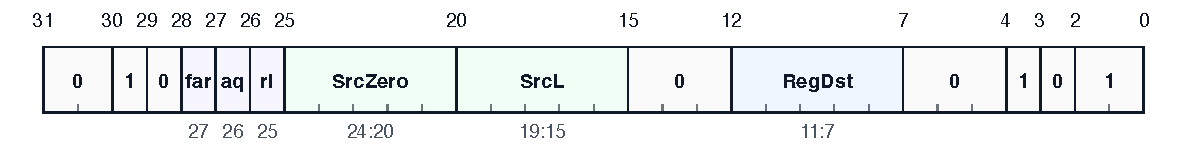
\includegraphics[width=\textwidth]{figs/encoding/scalar_instruction_entries/enc_lr_w.pdf}\par\smallskip
\begin{description}[leftmargin=0.18\linewidth,style=nextline]
\item[Format] \texttt{L32} \texttt{32-bit} scalar word.
\item[Pattern] \texttt{0010.............000.....0001011}.
\end{description}
\noindent\textbf{Classification.}\par
\begin{description}[leftmargin=0.18\linewidth,style=nextline]
\item[Category] Atomic Memory Operations.
\item[Family] Atomic Operation.
\item[Execution class] \texttt{AMO}; uop\_kind=AMO.
\end{description}
\noindent\textbf{Operand fields.}\par
\begin{description}[leftmargin=0.18\linewidth,style=nextline]
\item[\texttt{RegDst}] Bits \texttt{11:7 (5b)}. 5-bit scalar destination register that receives the original memory value returned by the atomic operation; X0 discards the returned value.
\item[\texttt{SrcL}] Bits \texttt{19:15 (5b)}. 5-bit scalar source register containing the memory address for the load-reserved operation.
\item[\texttt{SrcZero}] Bits \texttt{24:20 (5b)}. 5-bit source-register field that must encode X0; it occupies the standard source slot for encodings that do not consume a second register operand.
\item[\texttt{aq}] Bits \texttt{26:26 (1b)}. Acquire ordering bit for atomic memory operations. When set, later memory operations cannot be observed before this operation in the selected ordering domain.
\item[\texttt{far}] Bits \texttt{27:27 (1b)}. Atomic ordering-domain qualifier used with aq/rl suffixes; the assembly suffix containing f selects this encoded bit.
\item[\texttt{rl}] Bits \texttt{25:25 (1b)}. Release ordering bit for atomic memory operations. When set, earlier memory operations cannot be observed after this operation in the selected ordering domain.
\end{description}
\noindent\textbf{Operation.}\par
\begin{lstlisting}[style=ptoscalarcode]
addr = Read(SrcL)
value = LoadReserved32 (addr)
Write(RegDst, value)
\end{lstlisting}
\Needspace{0.08\textheight}
